\begin{figure*}[t]
\centering
\small
\newcommand\antwidth{0.14}
\newcommand\humanoidwidth{0.14}
\subfloat[\texttt{Ant-length-mass} environment.]{
\begin{tabular}{c}
\addvbuffer[0pt 0pt]{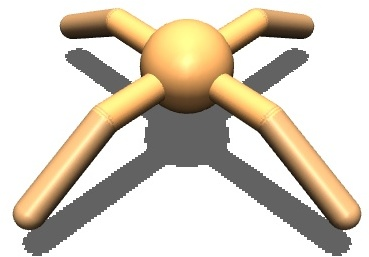
\includegraphics[width=\antwidth\textwidth, valign=m]{Figures/gym/ant_leg_length_mass_interp_0.00.jpg}} $\rightarrow$ \addvbuffer[0pt 0pt]{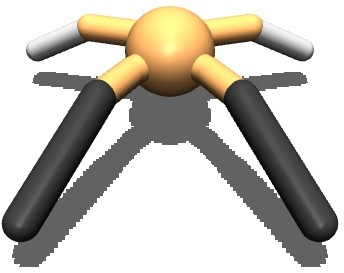
\includegraphics[width=\antwidth\textwidth,valign=m]{Figures/gym/ant_leg_length_mass_interp_1.00.jpg}}
\end{tabular} 
\label{fig:ant:length:mass}
} 
\hspace{5ex}
\subfloat[\texttt{Ant-length-mass} policy transfer experiment results. ]{
\begin{tabular}{l|c|c}
\hline
& TD3 & SAC \\ 
\hline
Expert on Source & 6826.52 & 6985.90 \\
\specialrule{.12em}{.05em}{.05em}
From Scratch & 4644.09 $\pm$ 502.05 & 5908.51 $\pm$ 339.81 \\ \hline
Direct Transfer & 4903.77 $\pm$ 801.12 & 6194.55 $\pm$ 165.82 \\ \hline
SOIL & 4891.67 $\pm$ 819.18 & 6061.32 $\pm$ 1102.58 \\ \hline
\textbf{Ours} & \textbf{5903.28 $\pm$ 416.07} & \textbf{6473.21 $\pm$ 207.98} \\ \hline
\end{tabular} 
\label{tab:ant:length:mass}
} 
\\
\subfloat[\texttt{Humanoid-length-mass} environment.]{
\begin{tabular}{c}
\addvbuffer[0pt 0pt]{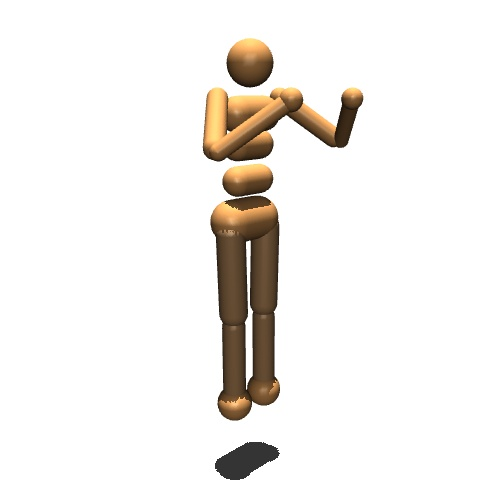
\includegraphics[height=\humanoidwidth\textwidth, valign=m]{Figures/gym/huamoid_leg_length_mass_interp_0.00.jpg}} $\rightarrow$ \addvbuffer[3pt 0pt]{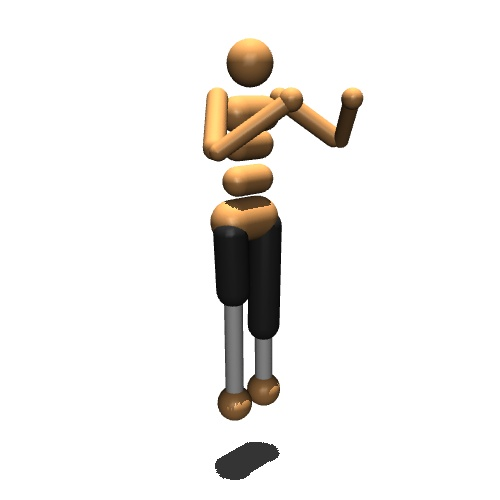
\includegraphics[height=\humanoidwidth\textwidth,valign=m]{Figures/gym/huamoid_leg_length_mass_interp_1.00.jpg}} 
\end{tabular} 
\label{fig:humanoid:length:mass}
} 
\hspace{5ex}
\subfloat[\texttt{Humanoid-length-mass} policy transfer experiment results. ]{
\begin{tabular}{l|c|c}
\hline
 & TD3 & SAC \\ 
\hline
Expert on Source & 6663.25 & 8271.70 \\
\specialrule{.1em}{.05em}{.05em}
From Scratch & 5824.07 $\pm$ 233.46 & 6468.60 $\pm$ 157.26 \\ \hline
Direct Transfer & 6256.15 $\pm$ 253.63 & 7639.61 $\pm$ 278.02 \\ \hline
SOIL & 6414.25 $\pm$ 505.79 & 6970.15 $\pm$ 659.32 \\ \hline
\textbf{Ours} & \textbf{7386.44 $\pm$ 151.24} & \textbf{7986.97 $\pm$ 129.21} \\ \hline
\end{tabular}
\label{tab:humanoid:length:mass}
} 
\\
\subfloat[\texttt{Ant-leg-emerge} environment.]{
\begin{tabular}{c}
\addvbuffer[0pt 0pt]{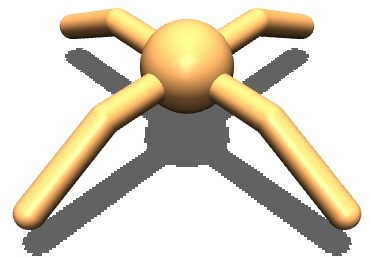
\includegraphics[width=\antwidth\textwidth, valign=m]{Figures/gym/ant_leg_emerge_interp_0.00.jpg}} $\rightarrow$ \addvbuffer[3pt 0pt]{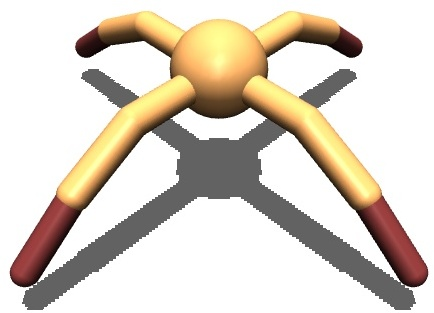
\includegraphics[width=\antwidth\textwidth,valign=m]{Figures/gym/ant_leg_emerge_interp_1.00.jpg}} \\
\end{tabular}
\label{fig:ant:leg:emerge}
} 
\hspace{5ex}
\subfloat[\texttt{Ant-leg-emerge} policy transfer experiment results.]{
\begin{tabular}{l|c|c}
\hline
& TD3 & SAC \\
\hline
Expert on Source & 6591.832 & 6431.32 \\
\specialrule{.1em}{.05em}{.05em}
From Scratch & 2551.30 $\pm$ 316.95 & 3845.69 $\pm$ 243.92 \\ \hline
Direct Transfer & 3579.40 $\pm$ 118.06 & 6031.27 $\pm$ 320.81  \\ \hline
SOIL & 1703.62 $\pm$ 351.83 & 4533.09 $\pm$ 578.32 \\ \hline
\textbf{Ours} &  \textbf{4688.68 $\pm$ 270.51} & \textbf{6612.78 $\pm$ 264.50} \\ \hline
\end{tabular}
\label{tab:ant:leg:emerge}
}
\caption{
\textbf{Experiments on source-to-target policy transfer on the MuJoCo Gym environments.}
All methods are trained for three million iterations with five different seeds. 
Mean and standard deviation of the reward of an epoch are reported. Our approach outperforms the baselines across different policy optimization schemes and across environments.
}
\label{fig:gym:combine}
\end{figure*}

